% Partie 1.3 - 6LoWPAN %

\subsection{6LoWPAN}

Cette partie à pour but de présenter le protocole 6LoWPAN ainsi que la norme 802.15.4 utiliser dans les couches basses de 6LoWPAN.

\subsubsection{802.15.4}

Ce standard de l'\textbf{IEEE} est définie sur 2 couches du \textbf{modèles OSI}, la couche physique et la couche MAC. Il est à la base de différents protocoles IoT (ZigBee notamment) qui implémentent des couches supérieurs différentes. 

Le framework de base prévoie un rayon de communication de 10 mètres pour un débit allant jusqu'à 250 kbit/s. Il est bien sur possible de réduire la puissance d'émission (le rayon) et de diminuer le débit pour réduire la consommation électrique. L'idée derrière cette réduction drastique est de quand même de conserver une bonne fiabilité.

Comme Wi-Fi (802.11), 802.15.4 utilise au niveau 2 \textbf{CSMA/CA} pour éviter les collisions et intègre plusieurs mécanisme pour la sécurisation des communications. Certains appareils peuvent aussi intégrer des modules d'optimisation de la consommation, de détection de la qualité de la liaison ainsi que la puissance de réception. 

Les appareils conforme à la norme 802.15.4 peuvent désormais se caler sur 3 bandes de fréquences :  868, 915 et 2450 MHz.

Le standard défini deux types de nœud :

le premier est le \textit{Full-Function Device} (FFD). Il peut servir de coordinateur dans le PAN tout comme il peut fonctionner en tant que simple nœud. Ils sont doté d'un module de communication qui permet de pouvoir retransmettre des trames (faire du routage).

Le second est le \textit{Reduced-Function Devices} (RFD). Ils sont prévues pour être extrêmement simple et possèdent peut de ressource. A cause de cela, il ne peuvent que communiquer avec les FFD et ne peuvent pas être les coordinateurs.

\subsubsection{6LoWPAN}



\begin{figure}[h]
\begin{center}
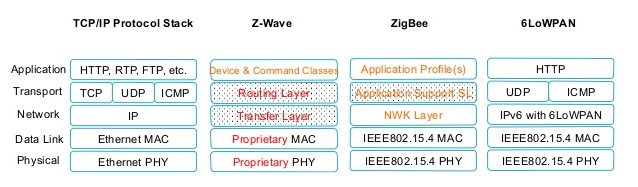
\includegraphics[width=15cm]{\rpDossier/images/comparison.jpg}
\end{center}
\caption{Comparaison de différents protocoles IoT}
\label{comparison}
\end{figure}
